\documentclass[a4paper,10pt,headings=normal,bibliography=totoc]{scrartcl}

\usepackage{scrhack}  % Fix a LaTeX warning

%%%%%%%%%%%%%%%%%%%%%%%%%%%%%%%%%%%%%%%%%%%%%%%%%%%%%%%%%%%%%%%%%%%%%%%%%%%%%%%
\usepackage[utf8x]{inputenc}
\usepackage{amsmath}
\usepackage{amssymb}
\usepackage{amsthm}
\usepackage{bm}
\usepackage{colonequals}
\usepackage{overpic}
\usepackage{url}
\usepackage{xspace}
\usepackage[square,numbers,sort]{natbib}

\usepackage[colorinlistoftodos,disable]{todonotes}
\usepackage{environ}
\usepackage{enumitem}
\usepackage{listings}
\usepackage{float}

%%%%%%%%%%%%%%%%%%%%%%%%%%%%%%%%%%%%%%%%%%%%%%%%%%%%%%%%%%%%%%%%%%%%%%%%%%%%%%%
%%%%%%%%%%%   hyperref should be loaded late to avoid incompatibilities
\usepackage[pdftitle={The dune-functions module},
            pdfauthor={Oliver Sander}]
             {hyperref}

\usepackage{attachfile2}
\usepackage{fancyvrb}

%%%%%%%%%%%%%%%%%%%%%%%%%%%%%%%%%%%%%%%%%%%%%%%%%%%%%%%%%%%%%%%%%%%%%%%%%%%%%%%
%%%%%%%%%%%%     Settings for the listings package
\lstset{language={c++},
         basicstyle=\ttfamily\small,
%         basicstyle=\small,
         commentstyle=\textit,
%         columns=fixed,
         columns=flexible,
         escapeinside={/*@}{@*/}
        }

% How to include ranges of an external source code file
\lstset{rangeprefix=//\ \{\ ,% curly left brace plus space, all in a C++-style comment
        rangesuffix=\ \},% space plus curly right brace
        numberstyle=\footnotesize,  % font size for numbers
        includerangemarker=false}  % Do not show the range markers

\newcommand{\cpp}[1]{\lstinline[basicstyle=\ttfamily]!#1!}

%%%%%%%%%%%%%%    Define a 'shellenv' environment for shell output
\usepackage{fancyvrb}

\DefineVerbatimEnvironment%
 {shellenv}{Verbatim}
 {}


%%%%%%%%%%%%%%%%%%%%%%%%%%%%%%%%%%%%%%%%%%%%%%%%%%%%%%%%%%%%%%%%%%%%%%%%%%%%%%%

\newcommand{\R}{\mathbb{R}}
\newcommand{\abs}[1]{{\lvert#1\rvert}}
\newcommand{\norm}[1]{\lVert#1\rVert}
\renewcommand{\div}{\operatorname{div}}
\DeclareMathOperator{\trace}{tr}

\newcommand{\dune}{\textsc{Dune}\xspace}
\newcommand{\program}[1]{\textsc{#1}\xspace}



% For typesetting Dune module names
\newcommand{\dunemodule}[1]{\texttt{#1}}
% For typesetting file names
\newcommand{\file}[1]{\texttt{#1}}


%%  All graphics files must be in this subdirectory
\graphicspath{{gfx/}}

%%%%%%%%%%%%%%%%%%%%%%%%%%%%%%%%%%%%%%%%%%%%%%%%%%%%%%%%%%%%%%%%%%%%%%%%%%%%%%%%%%%%%%%%%%%%%%%%%%%%%
%%%%%%%%%%%%%%%%%%%%%%%%%%%%%%%%%%%%%%%%%%%%%%%%%%%%%%%%%%%%%%%%%%%%%%%%%%%%%%%%%%%%%%%%%%%%%%%%%%%%%
%%%%%%%%%%%%%%%%%%%%%%%%%%%%%%%%%%%%%%%%%%%%%%%%%%%%%%%%%%%%%%%%%%%%%%%%%%%%%%%%%%%%%%%%%%%%%%%%%%%%%

\title{The dune-functions module}
\author{Oliver Sander}
%\date{}

\begin{document}

\maketitle

\begin{abstract}
 \dunemodule{dune-functions} is a \dune module that provides interfaces for functions and function space bases.
 It forms one abstraction level above grids, shape functions, and linear algebra, but still sits below
 full discretization frameworks like \dunemodule{dune-pdelab} and \dunemodule{dune-fem}.
 As an example, this document shows how the \dunemodule{dune-functions} module can be used to solve the Stokes
 equation with a Taylor--Hood discretization.
\end{abstract}


\section{Solving the Stokes equation with \dunemodule{dune-functions}}
\subsection{The Stokes equation}

\begin{figure}
 \begin{center}
  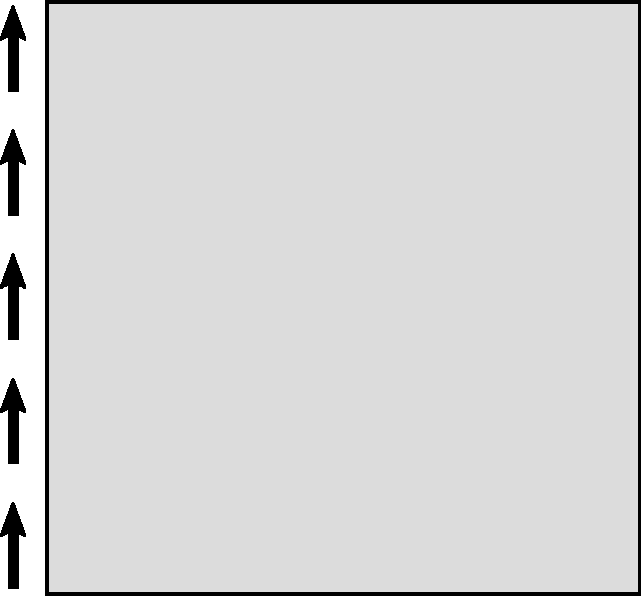
\includegraphics[height=0.3\textheight]{driven_cavity}
  \qquad
  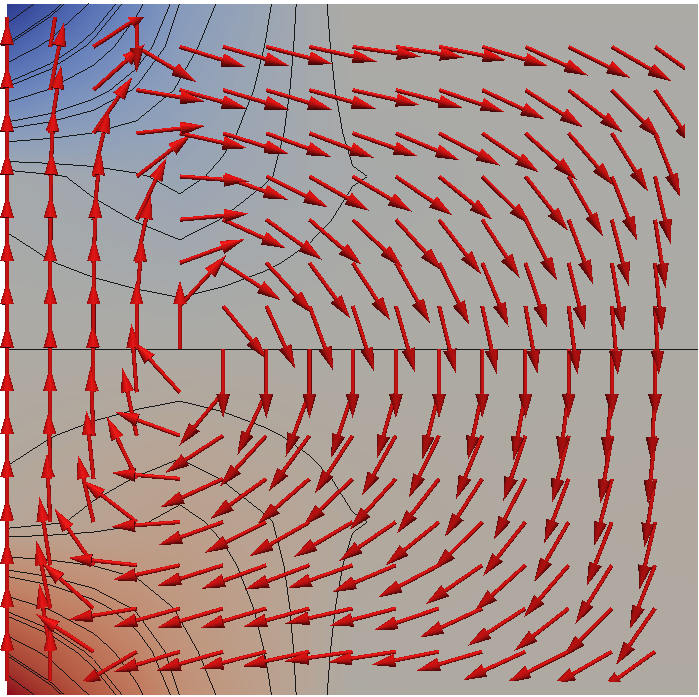
\includegraphics[height=0.3\textheight]{driven_cavity_result}
 \end{center}
 \caption{Driven cavity. Left: setting, right: simulation result.  The arrows show the {\em normalized} velocity.}
 \label{fig:dune_functions:driven_cavity}
\end{figure}

The Stokes equation models a viscous incompressible
fluid in a $d$-dimensional domain $\Omega$.  There are two unknowns in this problem: a stationary
fluid velocity field $\mathbf{u} : \Omega \to \R^d$, and the fluid pressure $p : \Omega \to \R$.
Together, they have to solve the boundary value problem
\begin{alignat*}{2}
 -\Delta \mathbf{u} - \nabla p & = 0  & \qquad & \text{in $\Omega$} \\
 \div \mathbf{u} & = 0                &        & \text{in $\Omega$} \\
                    \mathbf{u} & = \mathbf{u}_D  &        & \text{on $\partial \Omega$},
\end{alignat*}
where we have omitted the physical parameters.  The boundary value problem only determines the
pressure $p$ up to a constant function.  The pressure is therefore usually normalized such
that $\int_\Omega p\,dx = 0$.

Due to the constraint $\div \mathbf{u} = 0$, the corresponding weak form of the equation is a saddle-point problem.
Introduce the spaces
\begin{align*}
 \mathbf{H}^1_D(\Omega)
      & \colonequals
      \big\{ \mathbf{v} \in \mathbf{H}^1(\Omega) \; :\; \operatorname{tr}{\mathbf{v}} = \mathbf{u}_D \big\}, \\
 L_{2,0}(\Omega) & \colonequals  \Big\{ q \in L_2(\Omega) \; :\; \int_\Omega q\,dx = 0 \Big\},
\end{align*}
and the bilinear forms
\begin{equation*}
 a(\mathbf{u},\mathbf{v}) \colonequals \int_\Omega \nabla \mathbf{u} \nabla \mathbf{v} \,dx,
 \qquad \text{and} \qquad
 b(\mathbf{v},q) \colonequals \int_\Omega \div \mathbf{v} \cdot q \,dx.
\end{equation*}
Then the weak form of the Stokes equation is: Find $(\mathbf{u},p) \in \mathbf{H}_D^1(\Omega) \times L_{2,0}(\Omega)$ such that
\begin{alignat*}{2}
 a(\mathbf{u},\mathbf{v}) + b(\mathbf{v},p) & = 0 & \qquad & \text{for all $\mathbf{v} \in \mathbf{H}_0^1(\Omega)$} \\
 b(\mathbf{u},q)\qquad\qquad & = 0       &        & \text{for all $q \in L_{2,0}(\Omega)$}.
\end{alignat*}
If $\mathbf{u}_D$ is sufficiently smooth, this variational problem has a unique solution.
The Taylor--Hood element is the standard way to discretize this saddle point problem~\cite{braess:2013}.

\subsection{The driven-cavity benchmark}

For our example we choose to simulate a two-dimensional driven cavity.  This is a standard benchmark
for the Stokes problem in the literature.  Let $\Omega$ be the unit square $[0,1]^2$, and set the Dirichlet
boundary conditions for the velocity $\mathbf{u}$ to
\begin{equation*}
 \mathbf{u}(x)
 =
 \begin{cases}
  (0,1) & \text{if $x \in \{0\} \times [0,1]$} \\
  (0,0) & \text{elsewhere on $\partial \Omega$}.
 \end{cases}
\end{equation*}
The interpretation of this is a fluid container that is closed on all but one side.  While the fluid remains
motionless on the closed sides, an external agent drives a constant upward motion on the left vertical side.
The domain and boundary conditions are depicted in Figure~\ref{fig:dune_functions:driven_cavity}, left.
The corresponding solution is shown on the right side of the same figure.  The velocity forms a vortex,
while the pressure forms extrema in the two left corners.

In the following discussion we always use the letter $d$ to denote the space dimension, even though it is
known to be $d=2$ for our specific example.  This is to avoid confusion, because the number~2 also
appears a few times because we have two types of unknowns.

\subsection{Discretization}

\begin{figure}
  \begin{center}
   \begin{overpic}[width=0.5\textwidth]{taylor_hood_tree}
    \put(5,5){$P_2$}
    \put(30,5){$P_2$}
    \put(55,5){$P_2$}
    \put(87,31){$P_1$}
    \put(5,30){$V_\text{v}$}
    \put(5,57){$B_\text{TH}$}
    \put(30.7,32){$\otimes$}
    \put(61.6,58){$\otimes$}
   \end{overpic}

  \end{center}
  \caption{Taylor--Hood basis $P_2 \otimes P_2 \otimes P_2 \otimes P_1$ in a tree representation}
    \label{fig:taylor_hood_basis_tree}
\end{figure}

We discretize the domain using a structured axis-aligned grid with $4 \times 4$ uniform quadrilateral elements.
On this grid, we use the Taylor--Hood element to discretize the weak saddle-point problem.  The nodal basis
of the Taylor--Hood element has a natural tree structure as shown in Figure~\ref{fig:taylor_hood_basis_tree}.
On each element, the \dunemodule{dune-functions} implementation provides a local numbering of all shape functions
on this element.  This numbering uses a simple integer as index type, and is used to address the entries of the
element stiffness matrix.

\begin{table}
 \begin{center}
 \begin{tabular}{c|c}
 basis function & multi-index \\
 \hline \\
  $b_{x,0}$  & $(0,0)$ \\
  $b_{y,0}$  & $(0,1)$ \\
  $b_{z,0}$  & $(0,2)$ \\
  $b_{x,1}$  & $(0,3)$ \\
  $b_{y,1}$  & $(0,4)$ \\
  $b_{z,1}$  & $(0,5)$ \\
  $b_{x,2}$  & $(0,6)$ \\
  $b_{y,2}$  & $(0,7)$ \\
  $b_{z,2}$  & $(0,8)$ \\
    \vdots   & \vdots  \\
  $p_0$      & $(1,0)$ \\
  $p_1$      & $(1,1)$ \\
  $p_2$      & $(1,2)$ \\
    \vdots   & \vdots
 \end{tabular}
 \end{center}
 \caption{Multi-index for the Taylor--Hood basis with interleaved ordering of the velocity basis functions}
 \label{tbl:th_multiindices_interleaved}
\end{table}

Each global basis function additionally gets a global index, used to address the entries of the global stiffness
matrix.  In principle, \dunemodule{dune-functions} provides several types of orderings and multi-indices here.
The one that is used in the code example is given  in Table~\ref{tbl:th_multiindices_interleaved}: Each global
index is a pair $(a,b)$, where $a \in \{0,1\}$ switches between velocity and pressure basis functions,
and $b \in \mathbb{N}$ selects a particular basis function in either the set of velocity basis functions
or the set of pressure basis functions.


\subsection{Implementation}

This chapter discusses an example implementation of the Stokes problem, using only \dunemodule{dune-functions}
and no higher-level modules.  The example is contained in a single file, which comes as part of the \dunemodule{dune-functions}
source tree, in \file{dune-functions/examples/stokes-taylorhood.cc}.  If you read this document in electronic form,
the file can also be accessed by clicking on the icon in the margin.%
%
\marginpar{\attachfile[author=The dune-functions team,
                       color = 1 0 0,
                       mimetype=text/plain,
                       description=Complete source code of the Stokes/Taylor-Hood example]
                       {../../examples/stokes-taylorhood.cc}}

\subsubsection{The \texorpdfstring{\cpp{main}}{main} method}

We begin discussing the example code by describing its \cpp{main} method.  This method begins by setting up MPI and the grid.
We pick \cpp{YaspGrid} for the structured $4 \times 4$ quadrilateral grid.  Note that there is the line
%
\lstinputlisting[linerange={using_namespace_dune_begin-using_namespace_dune_end},
                 numbers=left]{../../examples/stokes-taylorhood.cc}
%
at the top of the file, so this namespace is imported completely.  Additionally, everything in the \dunemodule{dune-functions}
module is in the namespace \cpp{Functions}.  This namespace is not imported; instead, the prefix \cpp{Functions::} is always
given explicitly.


%
\lstinputlisting[linerange={main_begin-grid_setup_end},
                 numbers=left]{../../examples/stokes-taylorhood.cc}
%
The \cpp{gridView} object is the flat finite element grid that we will use for
the computation.
On this grid view, we then set up the function space basis for the Taylor--Hood element.  This is as simple as
%
\lstinputlisting[linerange={function_space_basis_begin-function_space_basis_end},
                 numbers=left]{../../examples/stokes-taylorhood.cc}
%
For each element, the \cpp{taylorHoodBasis} object will give us the tree of shape functions, and the corresponding local and global numberings.

Before being able to assemble the stiffness matrix of the Stokes system we need to pick suitable data structures
for the linear algebra.
The implementation of the Taylor--Hood basis selected in Line~\ref{li:stokes_taylorhood_select_taylorhoodbasis} orders the
velocity degrees of freedom before the pressure degrees of freedom.  Further, the velocity
components are interleaved.  The indexing scheme results from grouping degrees of freedom at the
tree root.  The resulting multi-indices all have length~2, and are given in Table~\ref{tbl:th_multiindices_interleaved}.
Consequently, the appropriate vector type is a pair of scalar vectors, one for the velocity and one for the pressure
degrees of freedom.  Analogously, the matrix must consist of $2 \times 2$ large sparse scalar matrices.
The following code sets up vector and matrix types for this, using the nesting machinery from \dunemodule{dune-istl}.
%
\lstinputlisting[linerange={linear_algebra_setup_begin-linear_algebra_setup_end},
                 numbers=left]{../../examples/stokes-taylorhood.cc}
%
Other index types are possible and possibly desirable here.  These would correspond to other vector and
matrix data types.

Now that we have chosen the C++ types for the matrix and vector data structures we can actually assemble the system.
Assembling the right-hand-side vector \cpp{rhs} is easy, because, apart from the Dirichlet boundary data (which we
will insert later), all its entries are zero.  An all-zero vector of the correct type and size is set up by the
following lines
%
\lstinputlisting[linerange={rhs_assembly_begin-rhs_assembly_end},
                 numbers=left]{../../examples/stokes-taylorhood.cc}
%
The \cpp{HierarchicVectorView} is a device that offers easier handling of arbitrarily nested vector data types.
In particular, it offers convenient resizing of an entire hierarchy of nested vectors.
The \cpp{taylorHoodBasis} object informs about the sizes of the corresponding finite element basis subtrees,
and Line~\ref{li:stokes_taylorhood_set_rhs_to_zero} fills the entire vector with zeros.

To obtain the stiffness matrix we first create an empty matrix object of the correct type.  The actual assembly
is factored out into a separate method.
%
\lstinputlisting[linerange={matrix_assembly_begin-matrix_assembly_end},
                 numbers=left]{../../examples/stokes-taylorhood.cc}
%
As the matrix assembly is the central part of this example we explain it in detail below, after having covered the \cpp{main} method.

Suppose now that we have the correct stiffness matrix assembled in the object \cpp{stiffnessMatrix}.  We still need
to modify the linear system to include the Dirichlet information.
In a first step we need to determine all degrees of freedom with Dirichlet data.  These are all the velocity degrees of freedom
on the domain boundary.  We could do this by using the \cpp{LocalKey} object of each basis function
to single out all those that are assigned to a boundary entity.  However, on a simple domain as the unit square
used here it is easier to use a geometric criterion.  We first define a predicate that returns \cpp{true}
if a given global coordinate \cpp{x} is on the domain boundary:
%
\lstinputlisting[linerange={boundary_predicate_begin-boundary_predicate_end},
                 numbers=left]{../../examples/stokes-taylorhood.cc}
%
The we interpolate this boolean-valued function in the space spanned by the velocity basis functions.
%
\lstinputlisting[linerange={interpolate_boundary_predicate_begin-interpolate_boundary_predicate_end},
                 numbers=left]{../../examples/stokes-taylorhood.cc}
%
Observe how the \dunemodule{dune-functions} interface allows to interpolate C++11 lambdas, which makes the code
very short and readable.  The expression \cpp{TypeTree::hybridTreePath(_0,i)} selects the different coordinate
directions of the velocity basis from the tree representation given in Figure~\ref{fig:taylor_hood_basis_tree}.
As the bases for the velocity components are all the same, an ordinary integer \cpp{i} is sufficient to choose
one of them.  In contrast, the velocity and pressure bases are different C++ types, and a compile-time
construction is needed to choose between them.  The object \cpp{_0} is defined in
\file{dune/typetree/utility.hh} as (roughly)
\begin{lstlisting}
std::integer_constant<std::size_t, 0> _0;
\end{lstlisting}
In the \cpp{TaylorHoodBasis} implementation, \cpp{_0} selects the velocity subtree and \cpp{_1} selects
the pressure subtree.

Finally, we define a function implementing the actual Dirichlet values function $\mathbf{u}_D$, and interpolate
that into the right-hand-side vector \cpp{rhs}.
%
\lstinputlisting[linerange={interpolate_dirichlet_values_begin-interpolate_dirichlet_values_end},
                 numbers=left]{../../examples/stokes-taylorhood.cc}
%
The expression \cpp{TypeTree::hybridTreePath(_0)} demands that only velocity degrees of freedom are
interpolated.  The \cpp{isBoundary} vector given as the last argument restricts the interpolation
to only the boundary degrees of freedom.

The stiffness matrix is modified in a more manual fashion.  For each Dirichlet degree of freedom we need to fill the corresponding matrix row
with zeros, and write a~1 on the diagonal.  As only velocity
degrees of freedom have Dirichlet values, we need to modify the two upper matrix blocks only.
%
\lstinputlisting[linerange={set_dirichlet_matrix_begin-set_dirichlet_matrix_end},
                 numbers=left]{../../examples/stokes-taylorhood.cc}
%
Finally, we can solve the linear system.  Efficiently solving the Stokes system is an art, which we do not want to
get into here.  Instead, we a GMRes solver, without any preconditioner at all.  This is known to converge,
albeit slowly.
\todo[inline]{Eigentlich peinlich.  Können wir nicht doch einen vernünftigen Löser nehmen?}
The advantage is that it can be written down in very few lines.
%
\lstinputlisting[linerange={stokes_solve_begin-stokes_solve_end},
                 numbers=left]{../../examples/stokes-taylorhood.cc}
%
Observe how the \cpp{RestartedGMResSolver} object is completely oblivious to the fact that the matrix
has a two-level nesting structure.  On the other hand, dedicated Stokes solvers usually operate
on some sort of Schur complement, and hence they need direct access
to the four submatrices.  This can be elegantly done using the nested matrix type
used for the stiffness matrix.

Once the iterative solver has terminated, we write the result to a VTK file.  For this, we write the resulting velocity as a vector field,
and the resulting pressure as a scalar field.  We subsample the grid twice, because the \cpp{VTKWriter}
class natively only displays piecewise linear functions.
%
\lstinputlisting[linerange={stokes_output_begin-stokes_output_end},
                 numbers=left]{../../examples/stokes-taylorhood.cc}
%
When run, this program produces a file called \file{function-stokes-result.vtu}.  The file can be opened in
\program{ParaView}, and the outcome looks like the image on the right in Figure~\ref{fig:dune_functions:driven_cavity}.

\subsubsection{The global assembler}

Now that we have covered the \cpp{main} method, we can turn to the assembler for the Stokes stiffness matrix.
As our main focus is the use of the \dunemodule{dune-functions} interfaces, the assembler
is the central part of our example.   We begin with the global assembler,
which is the routine \cpp{assembleStokesMatrix} called in Line~\ref{li:stokes_taylorhood_call_to_assemblestokesmatrix}
of the \cpp{main} method.
The global assembler sets up the matrix pattern, loops over all elements, and accumulates the element stiffness
matrices in the global matrix. The signature of the method is
%
\lstinputlisting[linerange={global_assembler_signature_begin-global_assembler_signature_end},
                 numbers=left]{../../examples/stokes-taylorhood.cc}
%
The only arguments it gets are the finite element basis and the matrix to fill.  Observe that the Taylor--Hood basis is not
hard-wired here, so we could call the method with a different basis.
However, not surprisingly the assembler for the Stokes problem makes relatively tight assumptions on the basis tree
structure, so relatively little practical freedom is possible here.  Ideally, a global assembler should be fully
generic, and all knowledge about the current spaces and differential operators should be confined to the local
assembler.  Real discretization frameworks like \dunemodule{dune-pdelab} do achieve this separation,
but for our example here we are less strict, to avoid technicalities.

The first few lines of the \cpp{assembleStokesMatrix} method set up the matrix occupation pattern, and initialize the matrix with zeros.
%
\lstinputlisting[linerange={setup_matrix_pattern_begin-setup_matrix_pattern_end},
                 numbers=left]{../../examples/stokes-taylorhood.cc}
%
The actual pattern assembly is implemented in a separate method \cpp{getOccupationPattern}.
It returns a $2 \times 2$ table of \cpp{MatrixIndexSet} objects.
\todo[inline]{Erklären?  Überspringen?  Anders implementieren?}
The four \cpp{BCRSMatrix} objects are initialized with these patterns in Line~\ref{li:stokes_taylorhood_setup_matrix_patterns}.
Line~\ref{li:stokes_taylorhood_set_matrix_to_zero}
fills the entire matrix with zeros.

Next comes the actual element loop.  We first request a \cpp{localView} object and a \cpp{localIndexSet} object
from the finite element basis:
%
\lstinputlisting[linerange={get_localview_begin-get_localview_end},
                 numbers=left]{../../examples/stokes-taylorhood.cc}
%
After that, we start the loop over the grid elements.  For each element, we bind the \cpp{localView} object
to the element and the \cpp{localIndexSet} object to
the \cpp{localView}.  From now on all enquiries to the local view and index set will implicitly refer to this element.
%
\lstinputlisting[linerange={element_loop_and_bind_begin-element_loop_and_bind_end},
                 numbers=left]{../../examples/stokes-taylorhood.cc}
%
We then create the element stiffness matrix, and call the separate method \cpp{getLocalMatrix} to fill.
By default, \dunemodule{dune-functions} supposes that the element stiffness matrix is dense and non-hierarchical,
and Line~\ref{li:stokes_taylorhood_select_element_matrix_type}
picks a suitable type for such a matrix.
%
\lstinputlisting[linerange={setup_element_stiffness_begin-setup_element_stiffness_end},
                 numbers=left]{../../examples/stokes-taylorhood.cc}
%
The \cpp{getLocalMatrix} method is discussed in detail below.
In addition to the \cpp{elementMatrix} object, it gets only the \cpp{localView} object.  This object contains
all necessary information.

Finally, we loop over the entries of the element stiffness matrix and add them onto the global matrix.
%
\lstinputlisting[linerange={accumulate_global_matrix_begin-accumulate_global_matrix_end},
                 numbers=left]{../../examples/stokes-taylorhood.cc}
%
The type returned in Lines~\ref{li:stokes_taylorhood_get_global_row_index} and~\ref{li:stokes_taylorhood_get_global_column_index}
for the global row and column indices is a multi-index.  It has length~2 for both velocity degrees of freedom and for
pressure degrees of freedom.  Observe how Line~\ref{li:stokes_taylorhood_scatter_matrix_indices} uses the length-2
multi-index to access the nested matrix type.  For vectors, this scattering of multi-indices is implemented
in general form in the \cpp{HierarchicVectorWrapper} class.

The preceding loops write in particular into the lower right matrix block, even though we know that for the Stokes
system this block contains only zeros.  A more optimized version of the code would leave out the lower right
submatrix altogether.

\subsubsection{The local assembler}

Finally, we investigate the method that assembles the element stiffness matrices.  Its signature is
%
\lstinputlisting[linerange={local_assembler_signature_begin-local_assembler_signature_end},
                 numbers=left]{../../examples/stokes-taylorhood.cc}
%
As you see, it only receives the local view of the Taylor--Hood basis, expected to be bound to an element,
and the empty matrix.
The first few lines of the method gather some information about the element the method is to work on.
In particular, from the \cpp{localView} object it extracts the element itself, and the element's dimension and
geometry
%
\lstinputlisting[linerange={local_assembler_get_element_information_begin-local_assembler_get_element_information_end},
                 numbers=left]{../../examples/stokes-taylorhood.cc}
%
Next, the element stiffness matrix is initialized.  The \cpp{localView} object knows the total number of
degrees of freedom of the element it is bound to, and since the matrix is scalar this is the correct
number of matrix rows and columns.
%
\lstinputlisting[linerange={initialize_element_matrix_begin-initialize_element_matrix_end},
                 numbers=left]{../../examples/stokes-taylorhood.cc}
%
Finally, we first ask for the set of velocity and pressure shape functions.
%
\lstinputlisting[linerange={get_local_fe_begin-get_local_fe_end},
                 numbers=left]{../../examples/stokes-taylorhood.cc}
%
The two objects are \cpp{LocalFiniteElement}s in the \dunemodule{dune-localfunctions} sense of the word.
In fact, they are objects of the
\cpp{LocalFiniteElementVirtualInterface} class.  The virtual interface of \dunemodule{dune-localfunctions} is used here
because the Taylor--Hood basis implementation accommodates grids with more than a single element type.

In Lines~\ref{li:stokes_taylorhood_get_velocity_lfe}--\ref{li:stokes_taylorhood_get_pressure_lfe} you see the tree structure of the Taylor--Hood basis in action again:
The expression
\begin{lstlisting}
localView.tree().child(_0,0)
\end{lstlisting}
returns the first child of the first child of the root, i.e., the basis for the $x_0$-component of the velocity field,
and
\begin{lstlisting}
localView.tree().child(_1)
\end{lstlisting}
is the basis for the pressure space.
As the root of the tree combines two different bases, we need to use the static identifiers \cpp{_0} and \cpp{_1}
from the \cpp{Dune::TypeTree::Indices} namespace to specify its children.  The inner node for the velocities
combines $d$ times the same basis, and hence the normal integer \cpp{0} can be used to address its first child.
Our implementation of the local Stokes assembler is actually ``cheating'', because it exploits the knowledge
that the same basis is used for all velocity components.  Therefore, only the first leaf of the velocity
subtree is acquired in Line~\ref{li:stokes_taylorhood_get_velocity_lfe}, and then used for all components.
Using separate local finite elements is wasteful because the same shape function values and gradients
would be computed multiple times.

Next, we construct a suitable quadrature rule and loop over the quadrature points.  The formula for the quadrature
order combines information about the element type, the shape functions, and the differential operator.
\todo[inline]{\cpp{QuadratureRuleKey} verwenden!}
%
\lstinputlisting[linerange={begin_quad_loop_begin-begin_quad_loop_end},
                 numbers=left]{../../examples/stokes-taylorhood.cc}
%
The quadrature loop starts like similar local assembler codes seen elsewhere.
First, we get the inverse transposed Jacobian
of the map from the reference element to the grid element, and the Jacobian determinant for the integral
transformation formula
%
\lstinputlisting[linerange={quad_loop_preamble_begin-quad_loop_preamble_end},
                 numbers=left]{../../examples/stokes-taylorhood.cc}
%
With these preparations done, we can assemble the first part of the stiffness matrix,  corresponding to the
velocity--velocity coupling.  For two $d$-valued velocity basis functions $\bm{\varphi}_i^k = \mathbf{e}_k \varphi_i$
and $\bm{\varphi}_j^l = \mathbf{e}_l \varphi_j$ we need to compute
\begin{equation*}
 a(\bm{\varphi}_i^k, \bm{\varphi}_j^l)
 =
 \int_\Omega \nabla \bm{\varphi}_i^k \nabla \bm{\varphi}_j^l \,dx
 =
 \delta_{kl} \int_\Omega \nabla \varphi_i \nabla \varphi_j \,dx,
\end{equation*}
where $\varphi_i$ and $\varphi_j$ are the corresponding scalar basis functions.
The code first computes the derivatives of the velocity
shape functions at the current quadrature point,
and then uses the matrix in \cpp{jacobian} to transform the shape functions gradients to
gradients of the actual basis functions defined on the grid element.
%
\lstinputlisting[linerange={velocity_gradients_begin-velocity_gradients_end},
                 numbers=left]{../../examples/stokes-taylorhood.cc}
%
Withe the velocity basis function gradients at hand we can assemble the velocity contribution
to the stiffness matrix.
%
\lstinputlisting[linerange={velocity_velocity_coupling_begin-velocity_velocity_coupling_end},
                 numbers=left]{../../examples/stokes-taylorhood.cc}
%
Noteworthy here are the Lines~\ref{li:stokes_taylorhood_compute_vv_element_matrix_row}--\ref{li:stokes_taylorhood_compute_vv_element_matrix_column} which,
for two given shape functions from the finite element basis tree, compute the flat lexicographic numbering
used to index the element stiffness matrix.  The expression \cpp{child(_0,k)} singles out the tree leaf
for the \cpp{k}-th component of the velocity basis.  The loop variables \cpp{i} and \cpp{j} run over
the shape functions in this set, and
\begin{lstlisting}
localView.tree().child(_0,k).localIndex(i);
\end{lstlisting}
returns the corresponding scalar index for this shape function in the set of {\em all} shape functions
of the Taylor--Hood basis on this element.  Line~\ref{li:stokes_taylorhood_update_vv_element_matrix} then updates the corresponding (scalar)
element matrix entry with the correctly weighted product the two gradients $\nabla \varphi_i$
and $\nabla \varphi_j$.

Once this part is understood, computing, the velocity--pressure coupling terms is easy.
For a given velocity shape function $\bm{\varphi}_i^k$ and pressure shape function $\theta_j$ we need
to compute
\begin{equation*}
 b(\bm{\varphi}_i^k,\theta_j)
 =
 \int_\Omega \operatorname{div} \bm{\varphi}_i^k \cdot \theta_j\,dx
 =
 \int_\Omega \sum_{l=1}^d \frac{\partial (\bm{\varphi}_i^k)_l}{\partial x_l} \cdot \theta_j\,dx
 =
 \int_\Omega \frac{\partial \varphi_i}{\partial x_k} \cdot \theta_j\,dx
 =
 \int_\Omega (\nabla \varphi_i)_k \cdot \theta_j\,dx.
\end{equation*}
As additional information we need the values of the pressure basis functions $\{\theta_j\}$ at the
current quadrature point.  These are evaluated by the following two lines:
%
\lstinputlisting[linerange={pressure_values_begin-pressure_values_end},
                 numbers=left]{../../examples/stokes-taylorhood.cc}
%
Then, the actual matrix assembly is
%
\lstinputlisting[linerange={velocity_pressure_coupling_begin-velocity_pressure_coupling_end},
                 numbers=left]{../../examples/stokes-taylorhood.cc}
%
Line~\ref{li:stokes_taylorhood_compute_vp_element_matrix_row} computes the flat lexicographic index of $\bm{\varphi}_i^k$,
and Line~\ref{li:stokes_taylorhood_compute_vp_element_matrix_column} computes the index for $\theta_j$ (remember that \cpp{_1} denotes
the pressure basis).  Finally, Lines~\ref{li:stokes_taylorhood_update_vp_element_matrix_a}--\ref{li:stokes_taylorhood_update_vp_element_matrix_b}
then add the resulting terms to the matrix.



\section{Interfaces for global function space basis}

We will now present the full interface provided by a global basis in
\dunemodule{dune-functions}. The interface decomposes in two parts:
The user interface and the implementors interface.

The user interface is what is exposed by an actual basis for use in
application code. Any basis satisfying this interface is a valid
global basis in the \dunemodule{dune-functions} sense.
The implementors interface describes the reusable part of
a basis which is given by a \emph{node-factory} in the following.
This interface allows to embed the node-factory into a function space
basis of a larger space. This can be used, e.g., to compose
ansatz bases for mixed formulations, multicomponent problems,
or coupled multi-physic problems.

In the next sections we will first describe the user interface
of a global basis and related classes. Then we describe the implementors
interface for node-factories and two special node-factories
that can be used to compose nested bases.
Finally we describe some convenience methods that simplify
the construction of composed bases for the user.



\subsection{User interface of a {\tt GlobalBasis}}
We now describe the user interface provided by global bases and related types.
Since there may be various implementations of those types, all class names used
below are auxiliary names.  We will group exported type names and related methods
to simplify the presentation.
In general each basis implementation may require its own specific data for construction.
Hence we do not enforce an argument list for this.

\begin{lstlisting}
class GlobalBasis
{
public:
  GlobalBasis(<implementation defined>);
\end{lstlisting}

As the global basis represents a function space defined on a grid view access to
the latter is provided by the {\tt gridView()} method while its type
is exported as {\tt GridView}. 

\begin{lstlisting}
  using GridView = <implementation defined>;
  const GridView& gridView() const;
\end{lstlisting}

One of the main functionalities of the global basis is to provide
access to the basis functions. The latter are available via the
local view interface. The {\tt localView()} method returns a new
object of type {\tt LocalView}. After binding this object to a
grid element from the respective grid view, it provides access
to the restriction of all basis functions whose support has a
nontrivial intersection with this element. For details on the
{\tt LocalView} interface see below.

\begin{lstlisting}
  using LocalView = <implementation defined>;
  LocalView localView() const;
\end{lstlisting}

All basis functions accessible via a bound local view have a
local index assigned to them. These local indices are zero-based,
consecutive, and unique within the respective element.
In order to  associate global degrees of freedom to basis functions
the local indices can be mapped to global indices. To facilitate
hierarchical representations of the basis these global indices
are in general multi-indices. The {\tt localIndexSet()} method
returns a new object of type {\tt LocalIndexSet} that, after
binding it to a local view, allows to map the local indices
of all basis functions appearing in this local view to those
global multi-indices. The interface of the {\tt LocalIndexSet}
is defined below.

\begin{lstlisting}
  using LocalIndexSet = <implementation defined>;
  LocalIndexSet localIndexSet() const;
\end{lstlisting}

The total number of basis functions of the global basis is
exported via the {\tt dimension()} method. However, since
the global indices are hierarchically structured multi-indices
of type {\tt MultiIndex}, this information is in general not
sufficient to allocate hierarchical containers for storing,
e.g., coefficients with respect to all basis functions.

Because of this, the basis provides access to the structural
information of those multi-indices via the {\tt size(SizePrefix)}
method. The given prefix takes the form of a multi-index itself.
For a prefix $(p_1,\dots,p_k)$ the method returns the maximal value $q$ such that there
is a global index of the form $(p_1,\dots,p_k,q-1,\dots)$.
If there is no such $q$ the result is undefined, unless
$(p_1,\dots,p_k)$ is itself one of the multi-indices.
In this case the result is zero.
In any case this corresponds to the number of direct children
of the node $(p_1,\dots,p_k)$ in the index tree.
For convenience there is also a method {\tt size()} returning the same
value the method with an empty prefix, i.e., {\tt size(\{\})}.

Since prefixes may have variable size, it is guaranteed that {\tt SizePrefix}
is always a {\tt Dune::ReservedVector<size\_type,k>} where {\tt k}
is strictly larger than the maximal length of a multi-index. The result
type of all size-related methods is exported as {\tt size\_type}.

\begin{lstlisting}
  using size_type = <implementation defined>;
  using SizePrefix = <implementation defined>;
  using MultiIndex = <implementation defined>;
  size_type dimension() const;
  size_type size() const;
  size_type size(const SizePrefix& prefix) const;
\end{lstlisting}

Finally, the basis exports its node-factory of type {\tt NodeFactory}
via the {\tt nodeFactory()} method. The concept of a node-factory
will be discussed below.

\begin{lstlisting}
  using NodeFactory = <implementation define>;
  const NodeFactory& nodeFactory() const;
};
\end{lstlisting}



\subsection{User interface of a {\tt LocalView}}
We will now continue with the description of the interface
of a local view as returned by {\tt GlobalBasis::localView()}.
Since a {\tt LocalView} is not meant to be constructed
manually, there is no interface for this. Instead, a {\tt LocalView}
can be obtained from the global basis via the {\tt localView()}
method. As a consequence the global basis of type {\tt GlobalBasis}
is known and exported by the {\tt globalBasis()} method.

\begin{lstlisting}
class LocalView
{
public:
  using GlobalBasis = <implementation defined>;
  const GlobalBasis& globalBasis() const;
\end{lstlisting}

A local view is meant to provides access to all basis
functions whose support has nontrivial intersection with
a given element. To achieve this, the local view must
first be bound to this element by calling {\tt bind(Element)}.
This call may incorporate expensive computations needed to
setup the those basis functions. The local view can be
bound to another element by calling this method again.
To set the local view to unbound state again, you
can call the {\tt unbind()} method.
Notice that the local view will store a copy of the bound
element that is accessible via {\tt element()}.

\begin{lstlisting}
  using GridView = typename GlobalBasis::GridView;
  using Element = typename GridView::template Codim<0>::Entity;
  void bind(const Element& e);
  const Element& element() const;
  void unbind();
\end{lstlisting}

The total number of basis functions associated to the
local view at the currently bound element is returned
by {\tt size()}. The result of calling this method in
unbound state is undefined.
To allow preallocation of buffers for local functions
the {\tt maxSize()} method returns the maximal of the
{\tt size()} method for all elements in the grid view
associated to the global basis. This can be called in
unbound state.

\begin{lstlisting}
  using size_type = typename GlobalBasis::size_type;
  size_type size() const;
  size_type maxSize() const;
\end{lstlisting}

Finally access to the actual basis functions is provided
by the {\tt tree()} method returning a reference to a
{\tt Tree} object. This encapsulates the basis functions
in a hierarchical tree structure to also represent structured
function spaces. The interface of the tree object is discussed
below.

\begin{lstlisting}
  using Tree = <implementation defined>;
  const Tree& tree() const;
};
\end{lstlisting}



\subsection{User interface of a local ansatz {\tt Tree}}
\subsection{User interface of a {\tt LocalIndexSet}}




\bibliographystyle{plainnat}
\bibliography{dune-functions-manual}

\end{document}

